\documentclass[final]{article}

\usepackage{APS360}
\usepackage{amsmath}
\usepackage[utf8]{inputenc}
\usepackage[T1]{fontenc}
\usepackage{hyperref}
\usepackage{url}
\usepackage{booktabs}
\usepackage{amsfonts}
\usepackage{nicefrac}
\usepackage{microtype}
\usepackage{xcolor}
\usepackage{graphicx}
\usepackage{caption}
\captionsetup{font=small,labelfont=bf}
\DeclareMathOperator{\sinc}{sinc}
\begin{document}
\vspace{-26pt}

\href{https://github.com/noshou/APS360/tree/main}{\textbf{Github Repo}}\hfill
\href{https://noshou.github.io/APS360/}{\textbf{Live Demo}}

%==============================================================================
\section{Brief Project Description}
%==============================================================================

Given a molecule's 3-D atomic coordinates and element identities as inputs, this
project predicts $I(q) \in \mathbb{R}^{|Q|}$, its X-ray scattering intensity curve, as
\emph{output} (Fig.~\ref{fig:arch}). $I(q)$ is a 1-D fingerprint of a molecule's 3-D shape,
used throughout structural biology and materials science. The exact calculation, the
Debye equation, sums every pairwise interatomic interaction and costs $O(N^2)$ in atom
count $N$; the fastest closed-form reduction (Stuhrmann's spherical-harmonic
decomposition, $O(N \cdot L^2)$) is what generates the ground-truth labels used here,
following the same spherical-harmonic approach as CRYSOL. Both are non-differentiable
analytic sums, not something that adapts to problem-specific structure. A graph neural
network, in the tradition of SchNet and directional message passing for molecular
property prediction, is well suited for three reasons: (1) atoms and their pairwise
interactions map naturally onto a graph's nodes and message passing, (2) message passing
gives a learned $O(N)$-per-round surrogate for the same underlying physics, cheap enough
to sit inside a differentiable pipeline (e.g. structure refinement by gradient descent on
predicted $I(q)$), and (3) the mapping from geometry to scattering curve is smooth and
highly structured, which is exactly what a GNN's inductive bias exploits.

\begin{figure}[h]
    \centering
    
\includegraphics[width=0.62\linewidth]{figs/architecture.png}
    \caption{Input (atomic coordinates + element types) $\to$ ScatterNet $\to$ output $\hat I(q)$.}
    \label{fig:arch}
\end{figure}

%==============================================================================
\section{Notable Contribution}
%==============================================================================

\subsection{Data Processing}

A dataset of 1,044,583 molecules spanning 1--6,046 atoms was assembled
from 13 sources (Table~\ref{tab:dataset}), covering 474 unique atom/ion types
(charge-resolved, e.g.\ \texttt{O} vs.\ \texttt{O2-}). Raw structures (\texttt{.cif},
\texttt{.pdb}, \texttt{.xyz}) were converted to a uniform Cartesian XYZ representation;
dummy/non-physical sites were removed, deuterium was mapped to hydrogen, zero-atom
structures were discarded, and non-element placeholders (\texttt{X}, \texttt{M},
\texttt{Cn}) were excluded from the ionic makeup.

\begin{table}[h]
\centering
\small
\caption{Cleaned dataset composition by source.}
\label{tab:dataset}
\begin{tabular}{lrl}
\toprule
Group & Molecules & Atom range \\
\midrule
COD (Crystallography Open Database)     & 532,302 & 1--6,032 \\
QM9 (small organic molecules)           & 133,844 & 3--29 \\
tmQM (transition metal complexes)       & 108,541 & 7--569 \\
rcsb\_sml (PDB, small)                  & 96,158  & 28--6,036 \\
viro3D (viral protein structures)       & 60,488  & 173--6,046 \\
hydration\_shells (water solvation)     & 48,571  & 3--147 \\
rcsb\_med (PDB, medium)                 & 31,749  & 2,996--6,046 \\
mofs (metal-organic frameworks)         & 30,863  & 10--5,760 \\
monoatomic clusters (6 metals)          & 1,282   & 2--380 \\
binary alloy clusters                   & 371     & 2--1,482 \\
Si/Ge clusters                          & 217     & 4--60 \\
Ar/Ne clusters                          & 127     & 2--55 \\
(NaCl)$_n$Cl$^-$ clusters               & 70      & 3--71 \\
\midrule
\textbf{Total} & \textbf{1,044,583} & \textbf{1--6,046} \\
\bottomrule
\end{tabular}
\end{table}

$I(q)$ ground truth was computed from the cleaned XYZ via the Stuhrmann decomposition at
$L{=}50$ and stored, together with the coordinates, in a compressed HDF5 database (ZFP
lossless for floating-point arrays, Bitshuffle+Zstd for metadata).

To avoid padding waste across a 1--6,046 atom size range, molecules are grouped by size
into 57 atom-count buckets (Fig.~\ref{fig:buckets}); each bucket is packed into batches
capped at a fixed atom budget, splitting further if it overflows that cap, and each
bucket is stratified 70/15/15 into train/val/test on its own, so every split contains
both small and large molecules.

\begin{figure}[h]
    \centering
    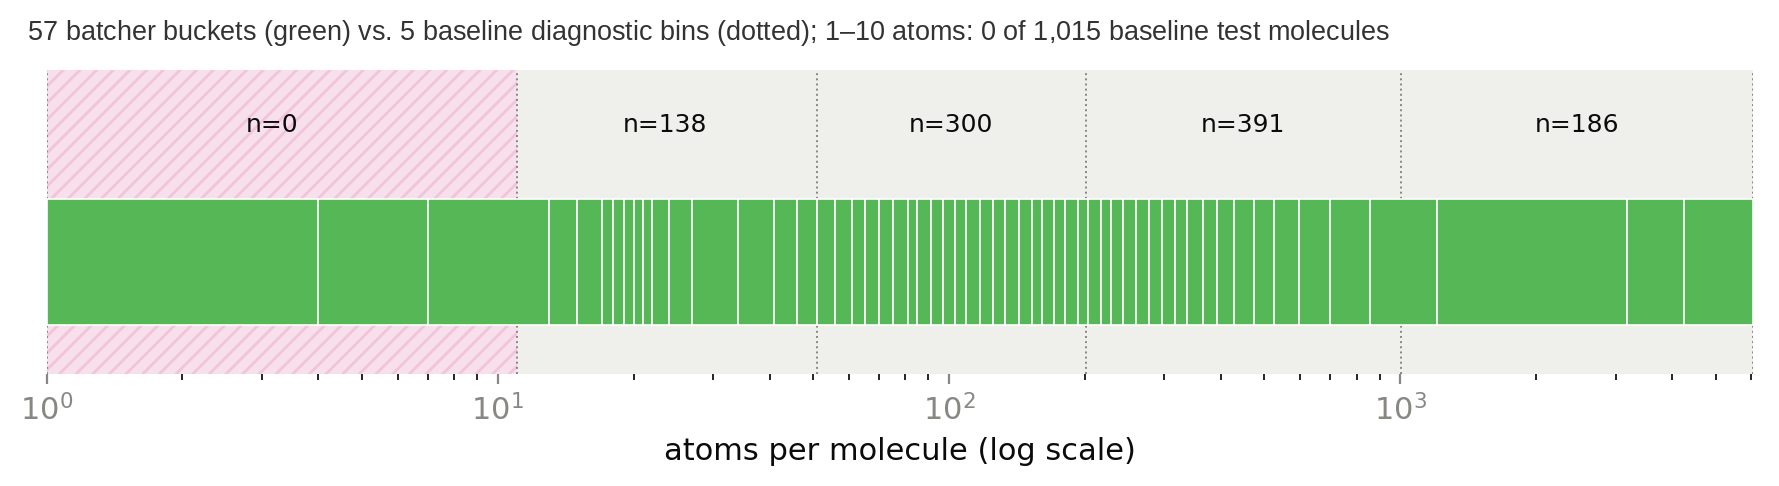
\includegraphics[width=\linewidth]{figs/bucket_distribution.png}
    \caption{The 57 training buckets (green) against the 5 coarse atom-count bins used to
    report baseline error by molecule size. The pink hatched bin ($n{=}0$) marks the
    1--10 atom range, where the baseline test slice happens to draw zero molecules, even
    though the training buckets themselves extend down to single atoms; the other four
    bins (shaded grey) each contain the baseline test molecules counted below their label.}
    \label{fig:buckets}
\end{figure}

There were many challenges with constructing the dataset due to data size, numerous
power outages that corrupted runs, and the weeks it took to calculate all the data.

\subsection{Baseline Model}

Nine non-GNN baselines were implemented: closed-form physics models fit per-molecule
(Guinier, Guinier-Porod, and a binned Debye sum evaluated over the histogrammed
pairwise-distance distribution $P(r)$, which recovers the exact Debye equation as the bin
count grows), stochastic estimators that subsample the $O(N^2)$ pairwise sum
(\texttt{propoEst}, \texttt{stratEst}), and learned baselines with no access to 3-D
geometry (a training-mean-by-atom-count lookup, a linear SVM over element-composition
features, and a 2-hidden-layer MLP over composition + size). Fig.~\ref{fig:baseline_summary}
reports the seven lowest-MSLE baselines (Guinier and Nearest-Neighbour diverge and are
omitted for readability).

\begin{figure}[h]
    \centering
    \begin{minipage}{0.44\linewidth}
        \centering
        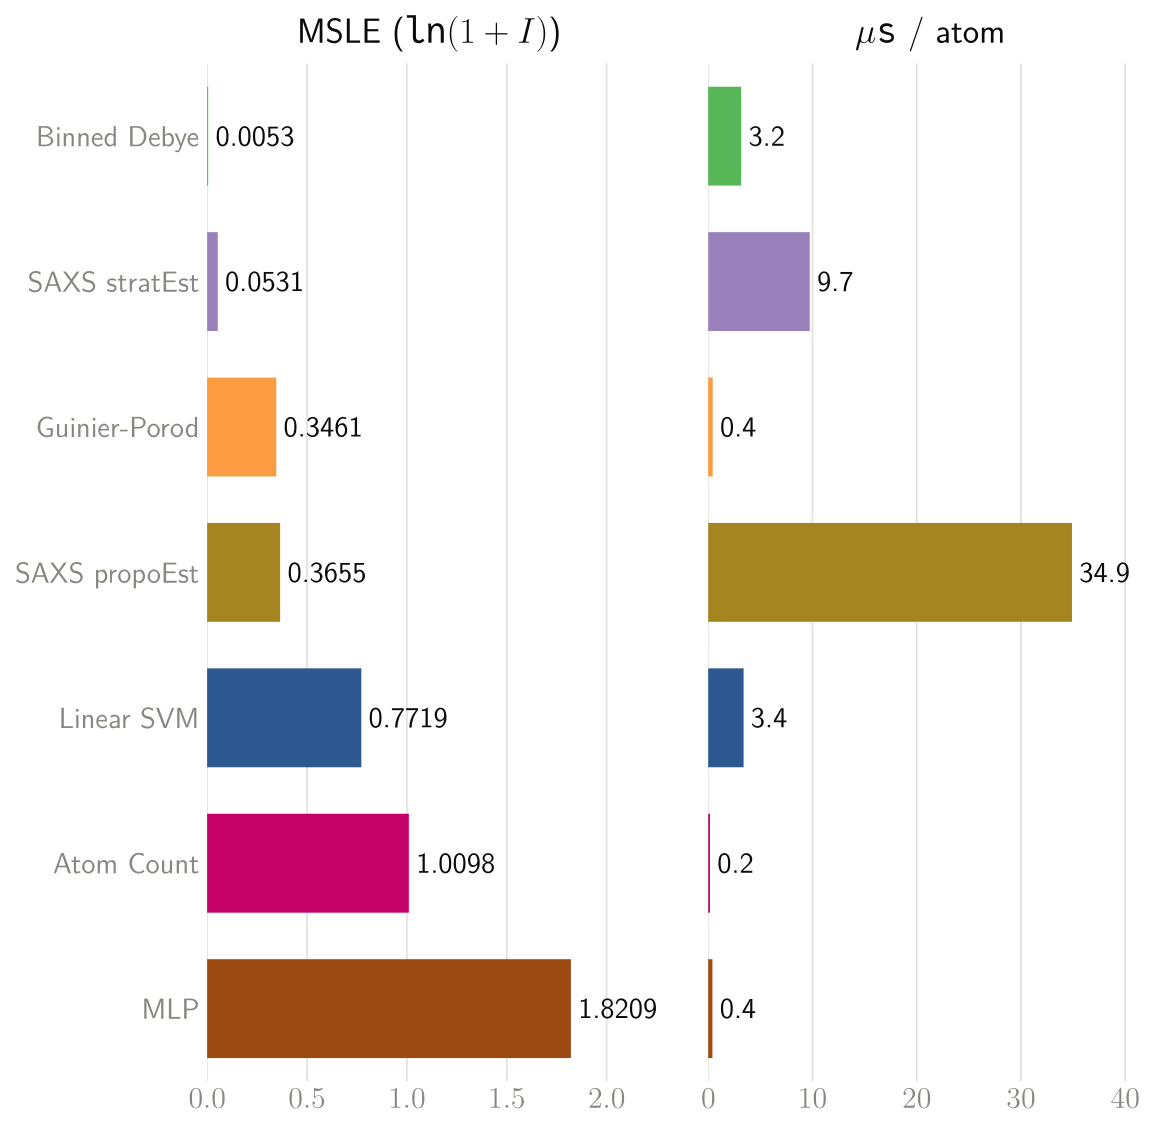
\includegraphics[width=\linewidth]{figs/baseline_summary_no_r2.png}
    \end{minipage}\hfill
    \begin{minipage}{0.52\linewidth}
        \centering
        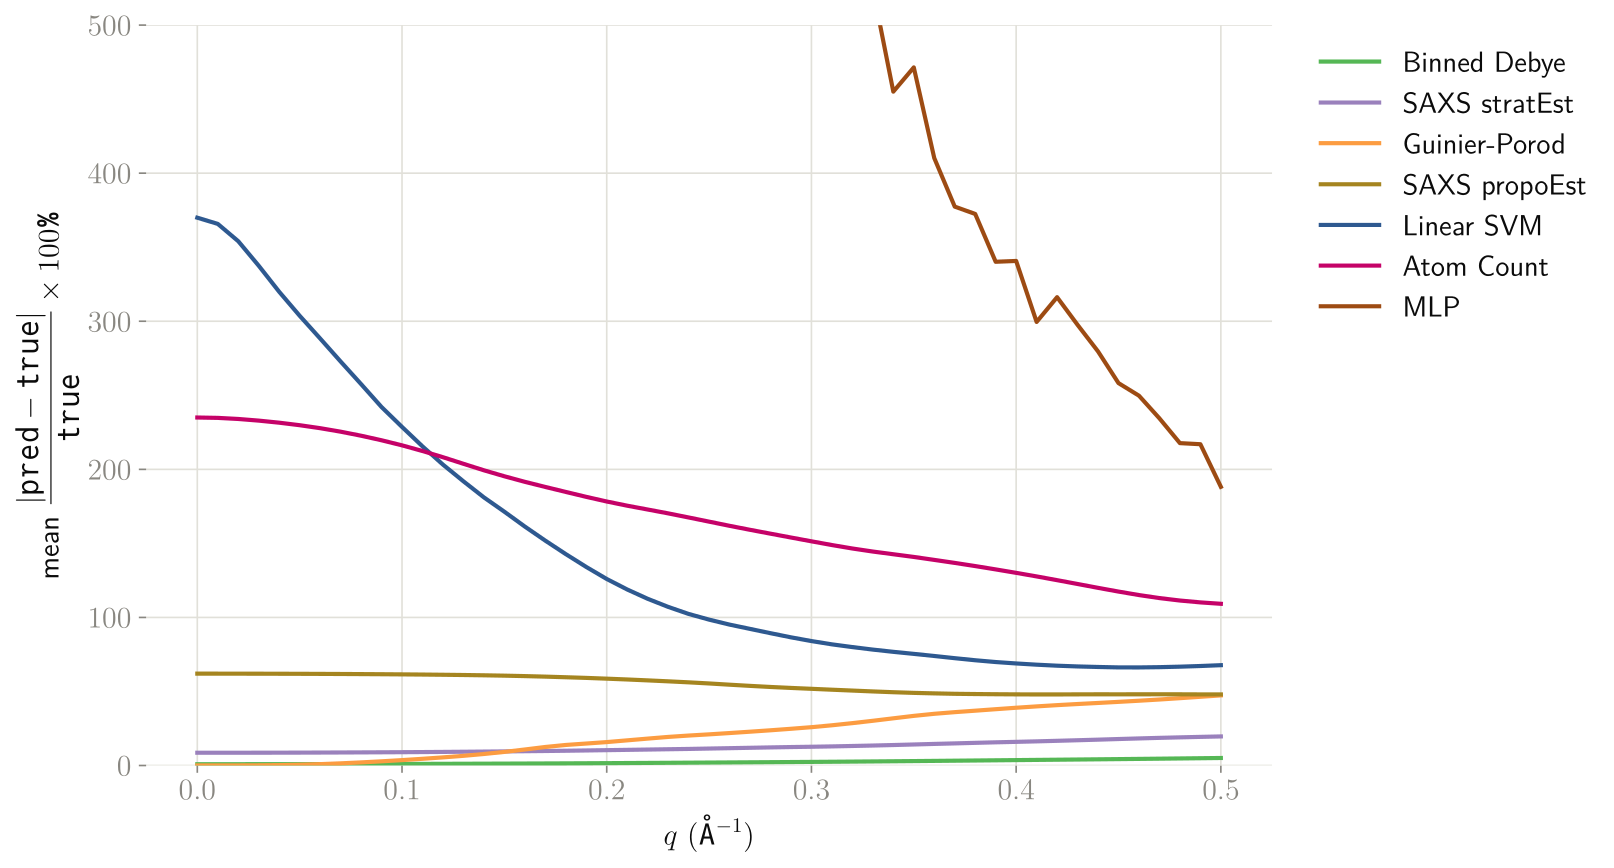
\includegraphics[width=\linewidth]{figs/baseline_per_q_percent_error.png}
    \end{minipage}
    \caption{Quantitative (left): MSLE and $\mu$s/atom, sorted by MSLE. Qualitative
    (right): per-$q$ mean percent error, baselines with explicit pairwise-distance
    information (Binned Debye, \texttt{stratEst}, \texttt{propoEst}) hold up best across
    the $q$-range; composition-only baselines (Atom-Count, Linear SVM, MLP) degrade
    earliest, since fine structural shape rather than overall size or composition
    determines $I(q)$ at mid-to-high $q$.}
    \label{fig:baseline_summary}
\end{figure}

Binned Debye is the strongest baseline (MSLE $0.0053$) since it is the closest
coarse-graining of the exact ground-truth formula, and is a useful feasibility ceiling
rather than a competitor to beat; the more informative comparison is against baselines
that, like the primary model, only see coordinates implicitly or not at all.
\textbf{Beating this baseline proves the model uses genuine 3-D structure, not just size
or composition:} the composition-only baselines -- Atom-Count, Linear SVM, and MLP --
are the lower bound, none of them accessing coordinates at all.
\textbf{Challenges:} \texttt{stratEst} segfaults on monoatomic molecules and both
stochastic estimators are noisy enough at small sample budgets to occasionally beat
their own asymptotic error, so their numbers should be read as a range rather than a
point estimate.

\subsection{Primary Model}

ScatterNet (Fig.~\ref{fig:arch}) has four stages. \textbf{Embed} looks up a learned
$\lambda_1{=}128$-d vector per atom, decomposed into a complex form factor magnitude
$|f_m(q)| = \mathrm{hypot}(f_0{+}f_1, f_2)$ (Cromer-Mann convention) and a bilinear
kernel bandwidth $\sigma_m(q)$. \textbf{MessagePass} ($\lambda_2{=}3$ rounds)
approximates the Gaussian kernel $k(\tilde r_i,\tilde r_j) = \exp(-\|\tilde r_i - \tilde
r_j\|^2/2)$, coordinates scaled by $\tilde r_m(q) = r_m/\sigma_m(q)$, via
$\lambda_5{=}64$ Random Fourier Features, reducing all-pairs aggregation from $O(M^2)$
to $O(M\lambda_5)$ per q-point. \textbf{OutputHead} is a $\lambda_4{=}4$-step halving MLP
at width $\lambda_3{=}128$ with a Softplus output, enforcing $\hat I(q) > 0$. The full
model has \textbf{427,352 parameters}, trained with a Kratky-weighted log-scale MSE plus
a form-factor penalty ($\lambda_6{=}0.1$) anchoring $\hat f_m(q)$ to the tabulated
xraydb reference and a $q^2$-weighted L2 penalty on $\sigma$ ($\lambda_7{=}0.1$)
preventing kernel-bandwidth blowup, via Adam, fp16, and tensor/data-parallel routing
across 2$\times$T4 GPUs (README \S7, \S12).

\begin{figure}[h]
    \centering
    \begin{minipage}{0.48\linewidth}
        \centering
        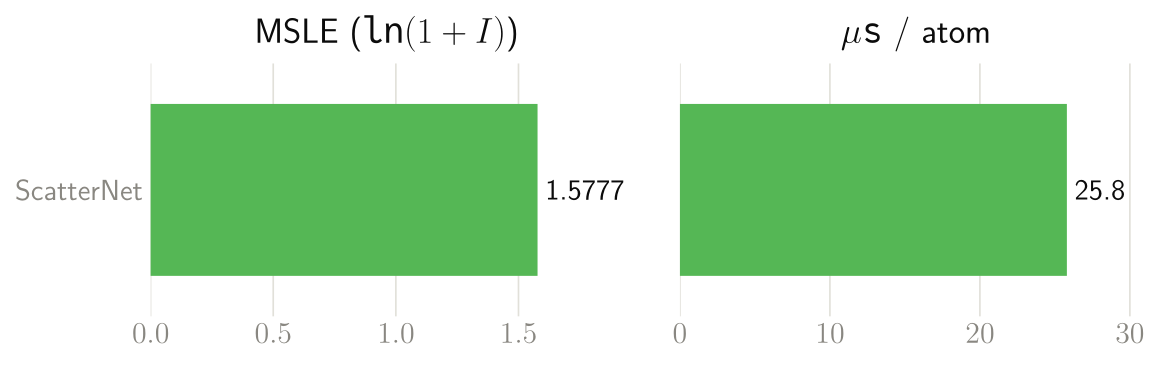
\includegraphics[width=\linewidth]{figs/scatternet_summary_no_r2.png}
    \end{minipage}\hfill
    \begin{minipage}{0.48\linewidth}
        \centering
        
\includegraphics[width=\linewidth]{figs/scatternet_per_q_percent_error.png}
    \end{minipage}
    \caption{ScatterNet, epoch 2 of 22 (dataset\_frac $=0.62$): quantitative summary
    (left) and per-$q$ mean percent error (right).}
    \label{fig:scatternet}
\end{figure}
\vspace{-14pt}

At epoch 2/22 (Fig.~\ref{fig:scatternet}), ScatterNet reaches MSLE $=1.578$ at 25.8
$\mu$s/atom inference, above every composition-only baseline (Fig.~\ref{fig:baseline_summary})
but still behind Linear SVM and the distance-aware physics/stochastic baselines, despite
having seen only $2/22 \times 0.62 \approx 5.6\%$ of the total training signal budget.
Error is concentrated in two places: percent error stays under 60\% for
$q>0.2$\,\AA$^{-1}$ but blows up at low $q$ (the large-scale/Guinier-region signal needs
the longest-range message passing to converge), and per-molecule MSLE falls
monotonically with atom count (10.7 for 1--10 atoms vs.\ 0.35 for 1001+).
\textbf{Feasibility:} loss is still falling steeply within epoch 2, and the
percent-error gap sits exactly where the physics baselines predicted (Guinier region,
Fig.~\ref{fig:baseline_summary}) -- evidence that continued training, not an
architecture change, is the primary path to closing the gap with the Binned Debye
ceiling. \textbf{Challenges:} tensor-parallel routing initially recompiled on every
eval-mode call due to shape mismatches with train-mode buckets; fixed by keying the
DP/TP routing decision on bucket shape alone (README \S7).

\end{document}
